% !TEX encoding = UTF-8 Unicode
%!TEX root = thesis.tex
% !TEX spellcheck = en-US
%%=========================================
\chapter{User Feedback Loop}

According to \cite{falconer2007cognitive}, we come up with the basic principles for the user feedback loop.
\begin{itemize}
	\item Provide ambiguous mappings to users, the application will detect the most ambiguous alignments and show them to users.
	\item Let users internally make mapping decisions and mark the decisions that users already made.
	\item User-driven navigation of concepts and properties for comparing.
	\item Search for a specific concept and to go back and forward for choosing the ambiguous alignments.
	\item Users can manually create mappings that are missed by the automated process.
\end{itemize}

%%=========================================
\section{Ambiguous Selection} % (fold)
\label{sub:ambiguous_selection}
In AgreementMaker, mappings are stored in a matrix data structure. We gather all the mapping matrices generated by different algorithms and select all different alignments. Those alignments are the ambiguous selections. We show the ambiguous selections with the matching confidence information to users and let them choose the best matching ones. Notices that even accurate matching algorithms cannot avoid incorrect matching, that is the reason to ask users to make decisions on ambiguous selections.

Fig.\ref{fig:url_degisn} shows the design of the URL panel and its workflow.

\begin{figure}[htb]
	\centering
	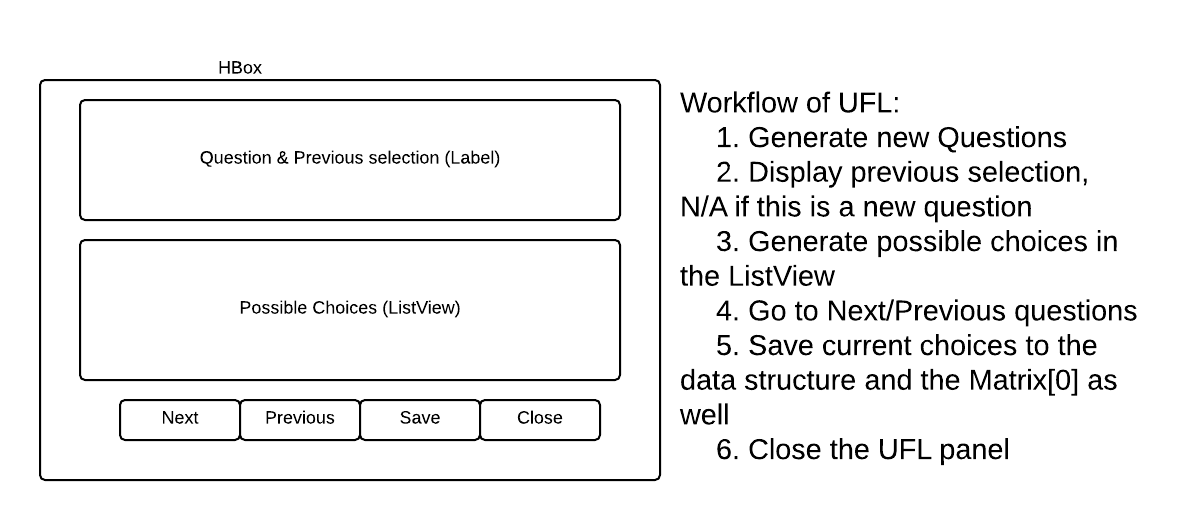
\includegraphics[width=3.5in]{pics/VA_UFL_Design.png}
	\caption{UFL design}
	\label{fig:url_degisn}
\end{figure}

Whenever the matching process finished, user is able to click on the UFL button and begin to see the ambiguous matching, then decide the better matching based on their own knowledge.

\begin{figure}[htb]
	\centering
	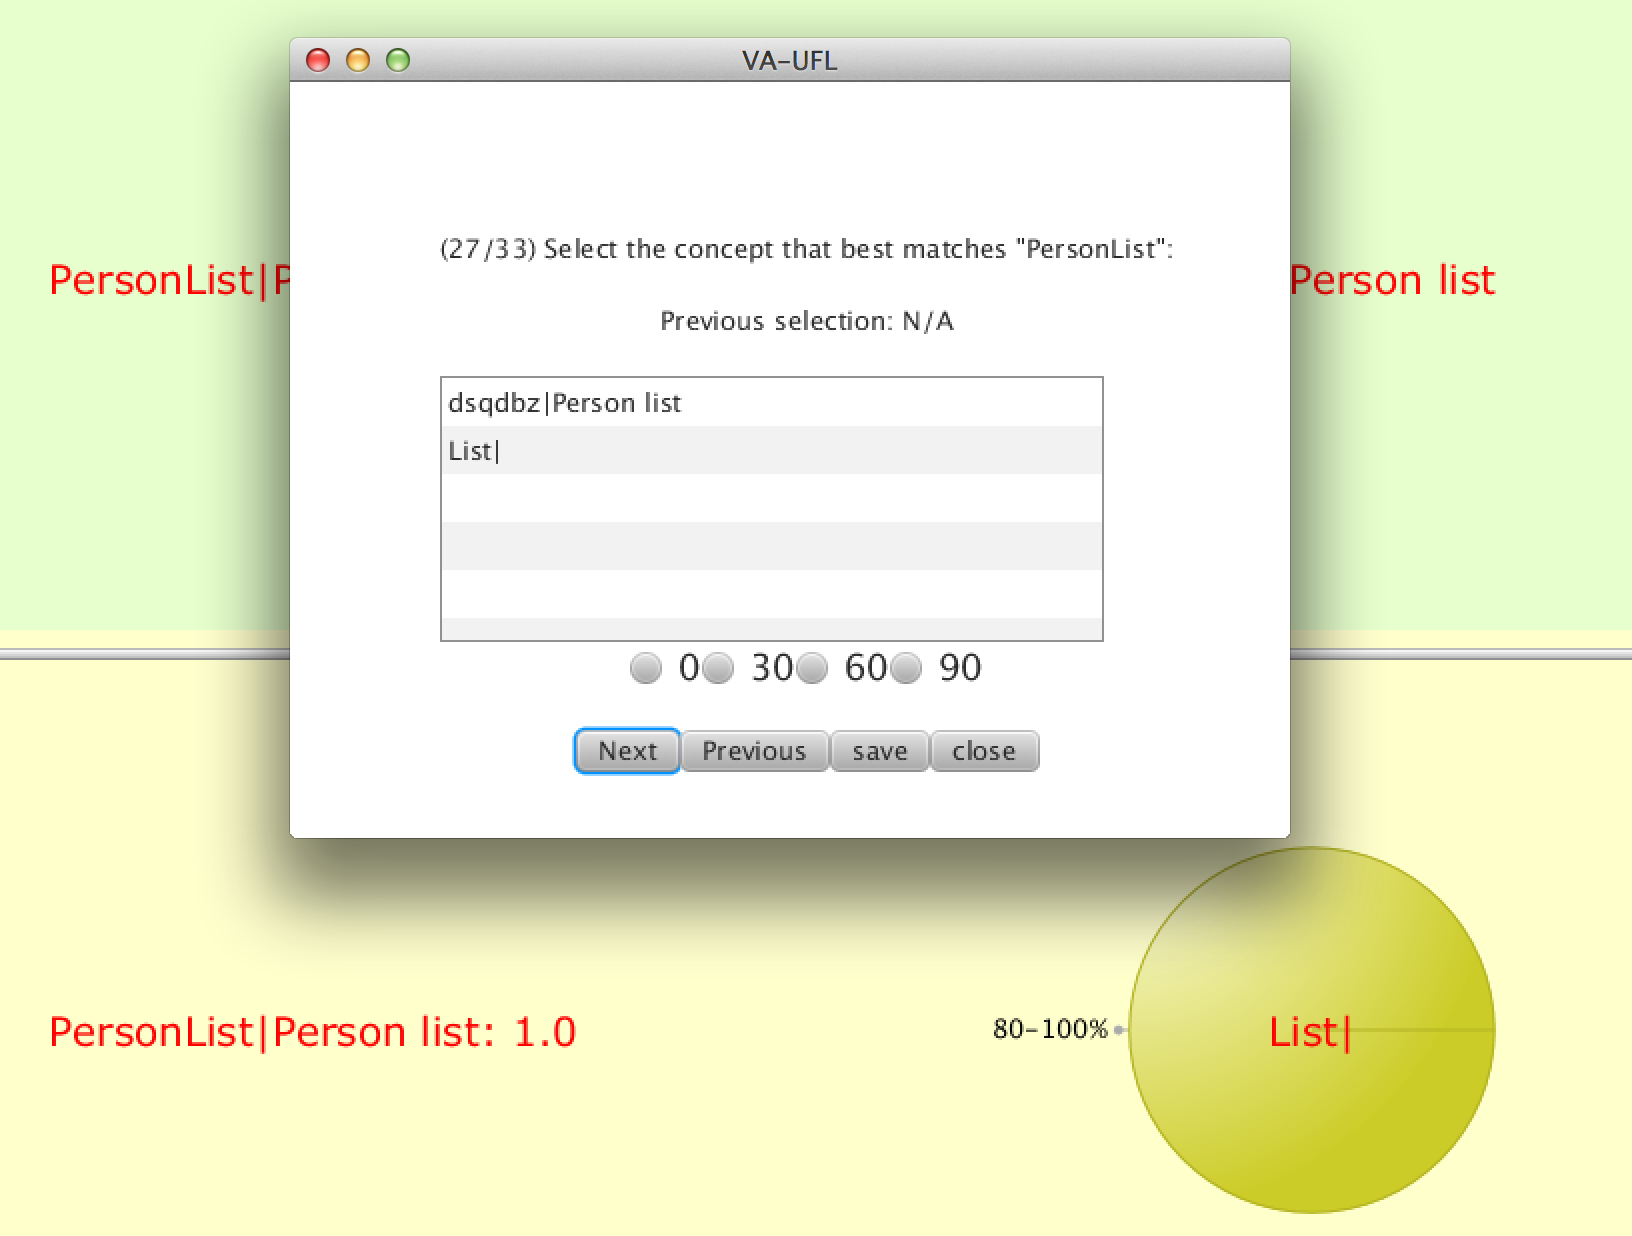
\includegraphics[width=3.5in]{pics/ufl.png}
	\caption{Ambiguous Selection}
	\label{fig:ambiguous_selection}
\end{figure}

%%=========================================
\section{Property Clustering} % (fold)
\label{sub:property_clustering}
Falcon-AO \cite{hu2008falcon} is a practical ontology matching system with acceptable to good performance and a number of remarkable features. PBM (Partition-based block matching) is one of the distinguishing features of Falcon-AO and it is a divide-and-conquer method for partition-based block matching that is practically applicable to large class hierarchies. Based on both structural affinities and linguistic similarities, two large class hierarchies are partitioned into small blocks respectively. Then, blocks from different hierarchies are matched based on the relatedness between them via anchors. PBM do the clustering based on the structural proximity, for example the distance between classes in the class hierarchy, and the overlapping between the domains of properties. In our user feedback loop, we can take the clustering idea as a reference. When comparing two matching results generated by different matching algorithms, we not only provide the matching similarities but also the properties that share the same domain of the two concepts. In this way, users will be able to see more valuable information. PBM generates clusters based on the overlapping between the domains of properties, in our user feedback loop we use the same idea to make clusters to help user better match the concepts by using their knowledge.\\

See Figure \ref{fig:property_clustering} for example. We use the anatomy datasets for testing purpose. We first load two ontologies, edas.owl (source ontology) and ekaw.owl (target ontology) and there is an ambiguous matching: 
\begin{itemize}
\item ConferenceEvent matches to Event with matching confidence 0.79 (matcher: Parametric String)
\item ConferenceEvent matches to Conference with matching confidence 0.61 (matcher: Vector-based Multi-words)
\end{itemize}

In the reference alignment the correct matching shows as 
\begin{itemize}
\item ConferenceEvent matches to Conference with matching confidence 1.00 
\end{itemize}
Before asking users to make choices, we generate floating panels to show users the properties. As we can see from Figure \ref{fig:property_clustering}, concept ConferenceEvent has properties hasAttendee, hasEndDateTime, hasLocation, hasProgramme and hasStartDateTime, those properties have the same domain as ConferenceEvent; concept Event has properties eventOnList, hasEvent, heldIn, organisedBy and partOfEvent, those properties have the same domain as Event; for concept Conference, there is no properties found. 

\begin{figure}[htb]
	\centering
	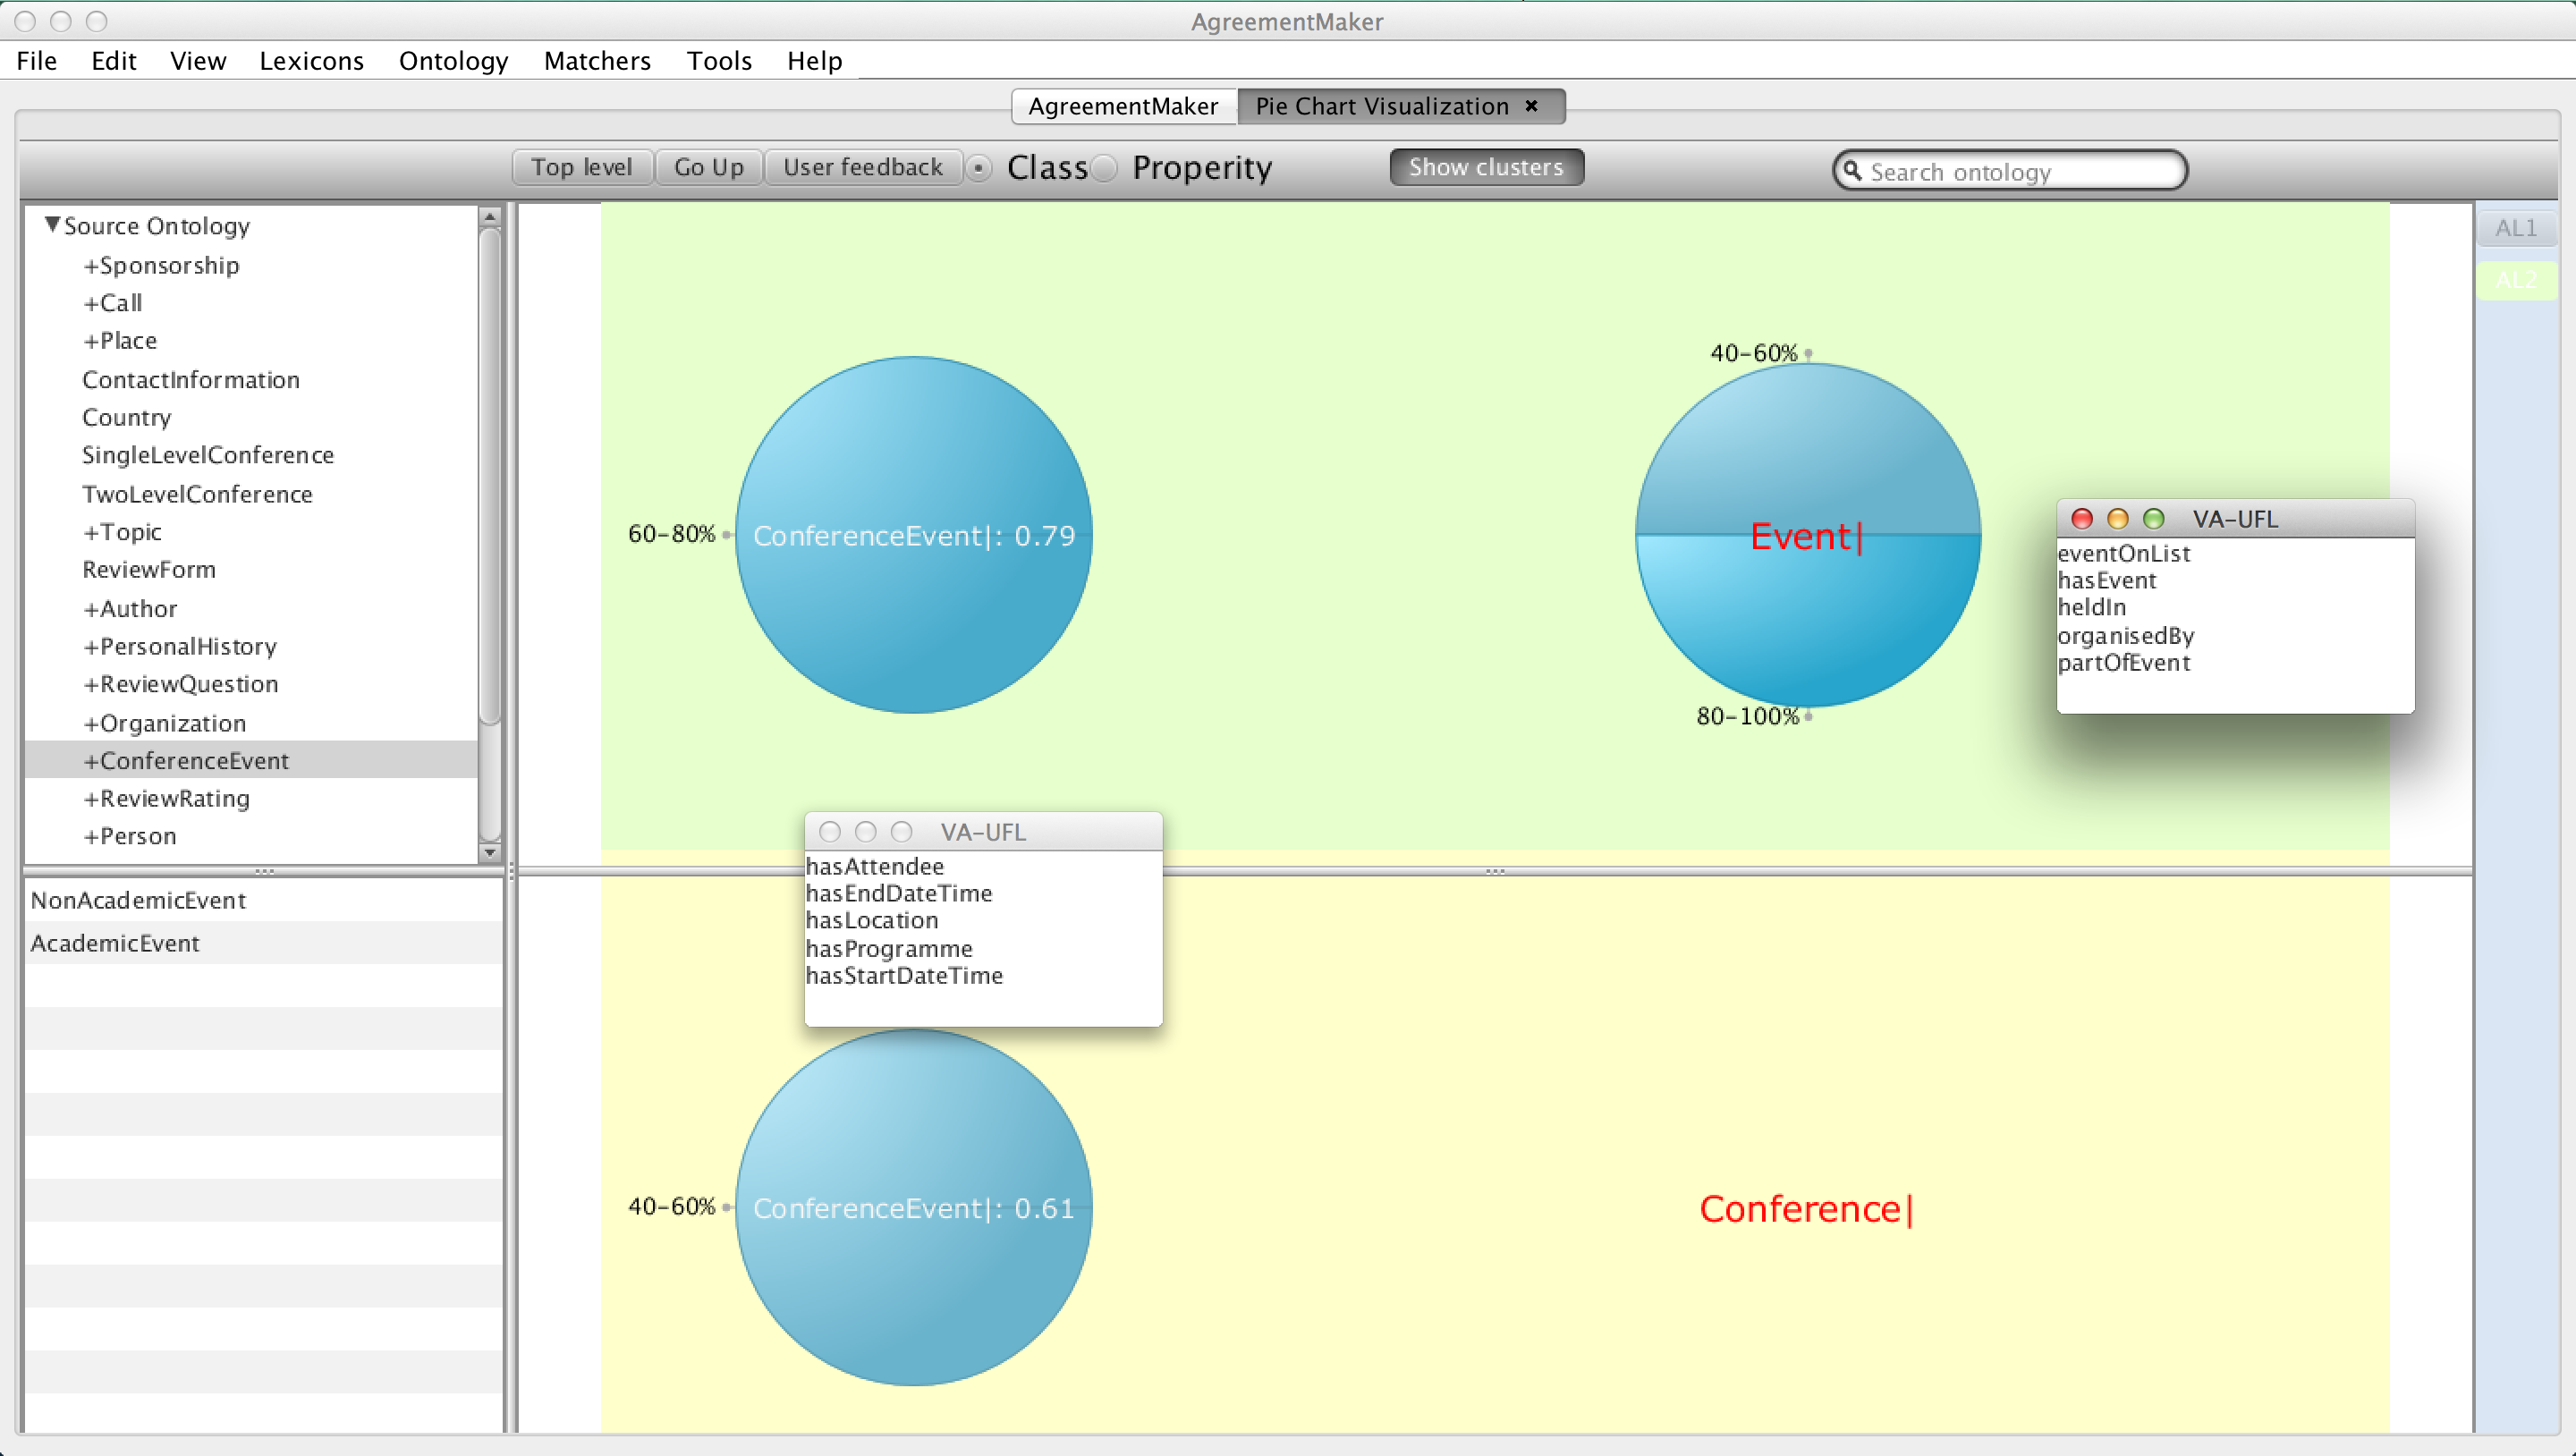
\includegraphics[width=6.5in]{pics/property_cluster.png}
	\caption{Property clustering}
	\label{fig:property_clustering}
\end{figure}

%%=========================================
\section{Integrating with AgreementMaker} % (fold)
\label{sub:integrating_with_agreementMaker}
In AgreementMaker, after executing the loaded algorithms, we first select the mapping result matrix with the highest matching similarity confidence. We make a copy of this matrix and regard it as the user defined matrix. Then we start the user feedback loop process and modify the user defined matrix with user selected alignments. 

\begin{figure}[htb]
	\centering
	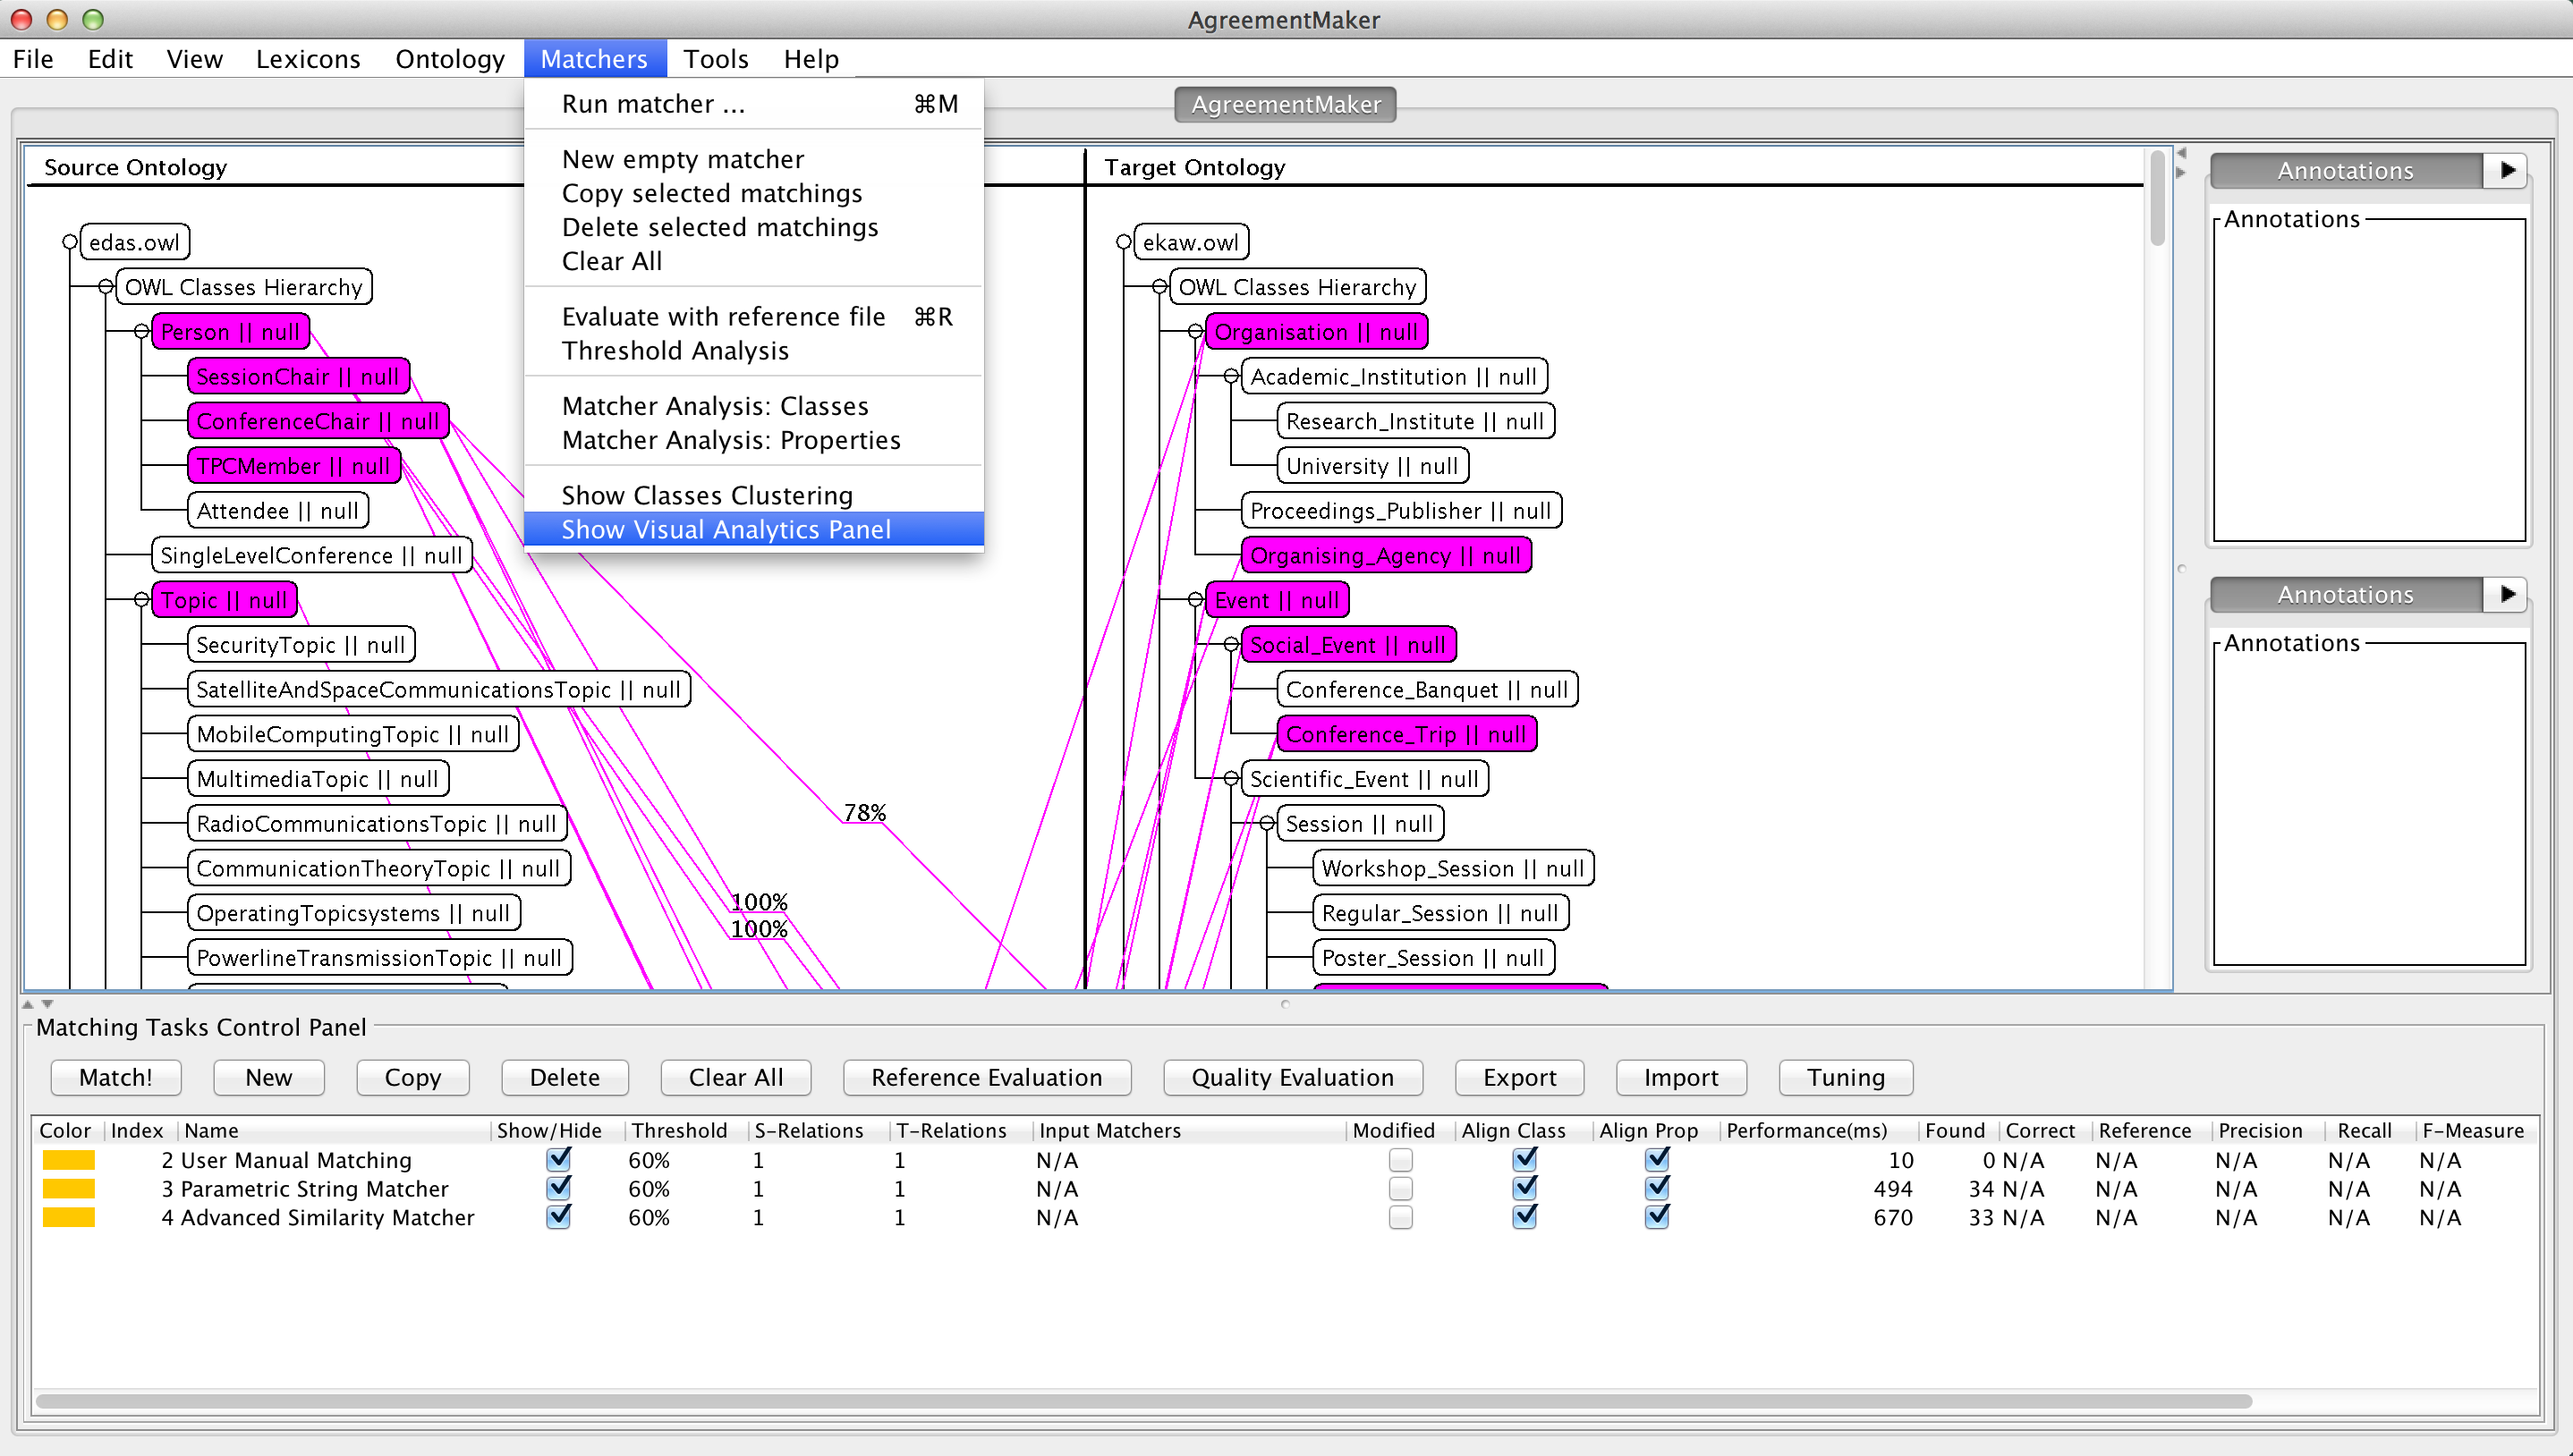
\includegraphics[width=6.5in]{pics/Integrate.png}
	\caption{Integrating with AM}
	\label{fig:integrating}
\end{figure}